\documentclass[12pt]{article}


\usepackage{amsmath}
\usepackage{amssymb}
\usepackage{attrib}
\usepackage{color}
\usepackage{fancyhdr}
\usepackage{graphicx}
\usepackage{hyperref}
\usepackage{makeidx}
\usepackage{stmaryrd}
\usepackage{xcolor}

\usepackage{preamble/lgarron-1.4.1}


\hypersetup{%
  colorlinks=true,% hyperlinks will be coloured
  linkcolor=blue,% hyperlink text will be green
  linkbordercolor=blue,% hyperlink border will be red
}

\def\rf{{\ \overset{R}\longleftarrow\ }}

\makeindex

\usepackage{multirow}

\usepackage{subfigure}
\usepackage{hhline}

\usepackage{fancyhdr}
\pagestyle{fancy}
\fancyhead[C]{SPCS Cryptography -- Homework 11}
\rhead{}

\lhead{}


\let\sol=\undefined
\newcommand{\sol}[1]{\begin{proof}\color{red}\textbf[SOLUTION: {#1}]\end{proof}}
%\newcommand{\sol}[1]{}


%%%%%%%%%%%%%%%%%%%%%%%%%%%%%%%%%%%%%%%%%%%%%%%%%%%%%%%%%%%%%%%%
  
\begin{document}

\section{Encryption}

Consider the following $PRP$:

$$
\begin{array}{c||c|c|c|c|c|c|c|c|c}
& 000 & 001 & 010 & 011 & 100 & 101 & 110 & 111 & m\\ \hhline{|=||=|=|=|=|=|=|=|=|=}
000 & 011 & 001 & 111 & 010 & 000 & 101 & 110 & 100 \\ \hline
001 & 101 & 110 & 010 & 000 & 111 & 100 & 001 & 011 \\ \hline
010 & 001 & 110 & 100 & 111 & 011 & 010 & 000 & 101 \\ \hline
011 & 101 & 011 & 100 & 111 & 110 & 000 & 010 & 001 \\ \hline
100 & 001 & 101 & 110 & 010 & 100 & 011 & 000 & 111 \\ \hline
101 & 000 & 001 & 010 & 011 & 100 & 110 & 101 & 111 \\ \hline
110 & 100 & 000 & 011 & 101 & 111 & 001 & 010 & 110 \\ \hline
111 & 110 & 101 & 001 & 011 & 111 & 000 & 010 & 100 \\ \hline
k
\end{array}
$$

\subsection{}

Check that this is a PRP (in particular, check that $F(k, x)$ is a permutation for any fixed key $k$).

\subsection{}

Use the to encrypt the following messages:

\begin{itemize}
\item {\tt 100} using CTR with IV $000$ and key $010$ \\\sol{{\tt 011}}
\item {\tt 100} using CBC with IV $000$ and key $010$ \\\sol{{\tt 110}}
\item {\tt 100} using OFB with IV $000$ and key $010$ \\\sol{{\tt 011}}
\item {\tt 011~010~101~100} using CTR with IV $100$ and key $010$ \\\sol{{\tt 101~000~110~101}}
\item {\tt 011~010~101~100} using CBC with IV $100$ and key $010$ \\\sol{{\tt 001~100~010~011}}
\item {\tt 011~010~101~100} using OFB with IV $100$ and key $010$ \\\sol{{\tt 101~001~001~010}}
\item {\tt 100~010~101~100} using CTR with IV $100$ and key $010$ \\\sol{{\tt 010~000~110~101}}
\item {\tt 100~010~101~100} using CBC with IV $100$ and key $010$ \\\sol{{\tt 111~010~001~010}}
\item {\tt 100~010~101~100} using OFB with IV $100$ and key $010$ \\\sol{{\tt 010~001~001~010}}
\item {\tt 011~010~101~100} using CTR with IV $010$ and key $010$ \\\sol{{\tt 111~110~011~110}}
\item {\tt 011~010~101~100} using CBC with IV $010$ and key $010$ \\\sol{{\tt 010~111~100~111}}
\item {\tt 011~010~101~100} using OFB with IV $010$ and key $010$ \\\sol{{\tt 111~100~110~000}}
\item {\tt 011~010~101~100} using CTR with IV $100$ and key $100$ \\\sol{{\tt 111~110~010~011}}
\item {\tt 011~010~101~100} using CBC with IV $100$ and key $100$ \\\sol{{\tt 111~100~111~110}}
\item {\tt 011~010~101~100} using OFB with IV $100$ and key $100$ \\\sol{{\tt 111~110~001~000}}
\end{itemize}


\section{}

\label{encrypt}

Pick a partner (someone new) and:

\begin{itemize}
\item Agree on a 3-bit key and padding scheme.

\item Ask them to send you a message that has between $7$ and $14$ bits, using CBC with a random IV.
\end{itemize}
 
\newpage

Recall that CBC-MAC is like CBC encryption, except with a constant IV and one extra PRP application at the end.

\begin{center}
\fbox{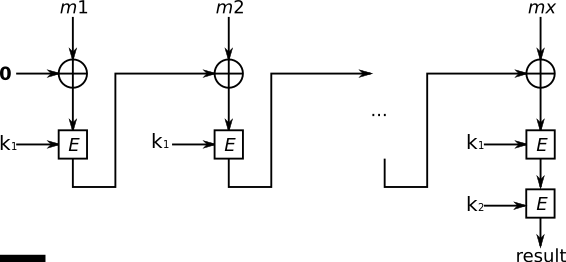
\includegraphics[width=10cm]{img/cbc-mac.png}}
\end{center}

\section{}

Calculate the MAC of {\tt 011~010~111~000} using CBC-MAC with keys $(k_1 = 010, k_2 = 011)$.

\sol{111 using the old homework.}

\section{CBC-MAC IV}


Suppose the IV for CBC-MAC were random instead of $0$. Would this help with security? Why/why not?

\sol{In theory, it would allow you to send the same message multiple times without giving away what the message is.

This is nice, but:
\begin{itemize}
\item It makes the message signature longer if you need to include the IV.
\item MACs are usually used to encrypted semantically secure cipher texts, which should be unique.
\end{itemize}

}

\section{}

The diagram above uses $k_2$ to encrypt the last block, instead of reusing $k_1$. What would happen if we allowed the same key to be used?

\sol{
Let ${\overline{0}}$ be the block of all zeros.

Ask for a signature

$$s = Sign\Big(k, {\overline{0}}\Big)$$

Output the following $3$-block message
$${\overline{0}}~\Big\|~{\overline{0}}~\Big\|~s$$
with the signature $s$.

Since this is a signature on a message we haven't seen, this is a forgery.


The ``trick'' is that $E(k, E(k  m))$

}

\section{MAC Security Game}

The idea behind the MAC security game is that:

\begin{itemize}
\item The adversary can ask for signatures on as many messages as (s)he wants, one at a time
\item The challenger replies with the signature on that message (using the secret key $k$).
\item The adversary wins if they output a message and a signature $(m, s)$ so that $Verify(k, m, s)$. (This is *different* from all the other security games we've seen so far).
\end{itemize}

Draw the diagram for this security game, and write the definition of advantage.

\section{}

Do the same as problem \ref{encrypt}, but also agree on keys $k_1, k_2$ for CBC-MAC and include the MAC with the message.

\section{MAC Forgery}

Suppose we didn't do the last encryption at the end, and allowed messages of any length to be encrypted. Show that we would lose security. In particular, show that someone with two valid message-signature pairs (using the same key[s]):

\begin{itemize}
\item $(m, s)$
\item $(m', s')$
\end{itemize}

can create a new message and a signature to go with it $(m'', s'')$ that verifies as valid.

(Hint 1: First, try this with the assumption that $m$ and $m'$ are one block each.)

(Hint 2: Try to place $m$ and $m'$ together, and use the output of the MAC to produce the same IVs during the CBC-MAC of the $m'$ portion as in the original $m'$ signature.)

\sol{

The signature $s = Sign(m, s)$ is the last block of the encryption of $m$.

Change the first block of $m'$ to $m'[0] \oplus s$ to produce $m^*$

$$
m^* = (m[0] \oplus s)~\Big\|~m[1]~\Big\|~m[2]~\Big\|~...
$$


Consider the encryption of the following:

$$
m' = m \Big\| m^*
$$
It will have the signature $s'$, so this allows us to produce a forgery.

}


\end{document}
